\documentclass{article}
\usepackage{graphicx}
\begin{document}
\section{Prvi del naloge}
Podatke razdelimo na train in test množico, hiperparametre nastavljamo na train množici, zaradi prekomernega prileganja. Poskusimo nekaj različnih algoritmov, spreminjamo parametre enega po enega: zvišujemo dokler se izboljšujejo z večjimi skoki, potem poskusimo manjše skoke za boljšo oceno. Najboljši rezultat je v RandomForestClassifier (RFC) z 80 sosedi.

Za avtomatiziran pristop preiskusimo tri algoritme: RFC, SVC in kNN. Številske parametre izbiramo enakomerno med smiselnimi vrednostmi, razen za parameter \verb|min_samples_split| (katerega izbiramo logenakomerno) in parameter \verb|gamma| in \verb|C| v SVC (izbiramo lognormalno). Poleg omenjenih nastavljamo v RFC: \verb|n_estimators| (med 32 in 200), \verb|max_depth| (med 2 in 32), \verb|criterion| (med gini, entropy in log\_loss); v SVC: \verb|shrinking| in tip jedra (sigmoid ali rbf); v kNN: \verb|n_neighbors| (med 2 in 256), \verb|weights| (uniform ali distance) in \verb|p| (1, 2, 3 ali 4).

Najboljša konfiguracija je algoritem RFC z \verb|criterion="log_loss"|, \verb|max_depth=29|, \verb|min_samples_split=20|, \verb|n_estimators=147|

Ne razumem navodila za četrto alinejo; konfiguracija, ki jo vrne hyperopt je samo ena. Prilagam slike za različne konfiguracije algoritmov iz (1.1).
\begin{figure}[h!]
    \caption{RandomForestClassifier}
    \centering
    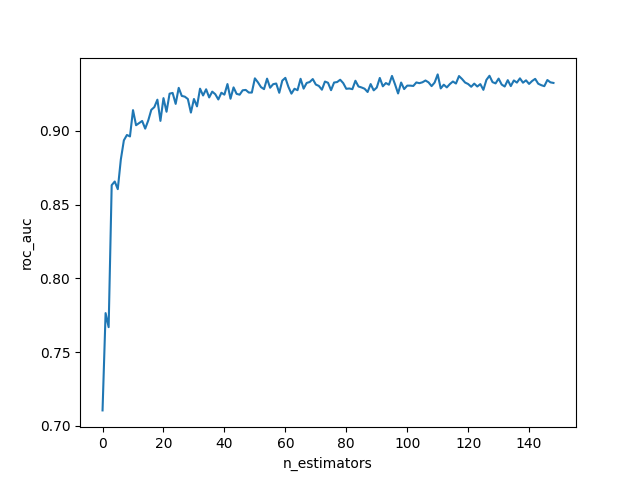
\includegraphics[width=0.8\textwidth]{rfc}
\end{figure}
\begin{figure}[h!]
    \caption{KNeighborsClassifier}
    \centering
    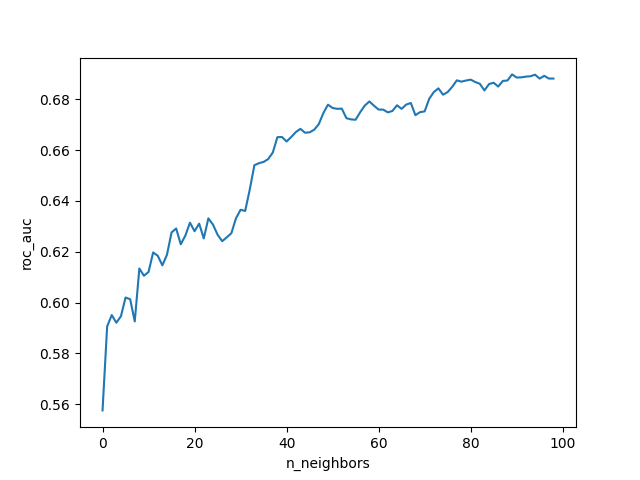
\includegraphics[width=0.8\textwidth]{knn}
\end{figure}
\begin{figure}[h!]
    \caption{SVC}
    \centering
    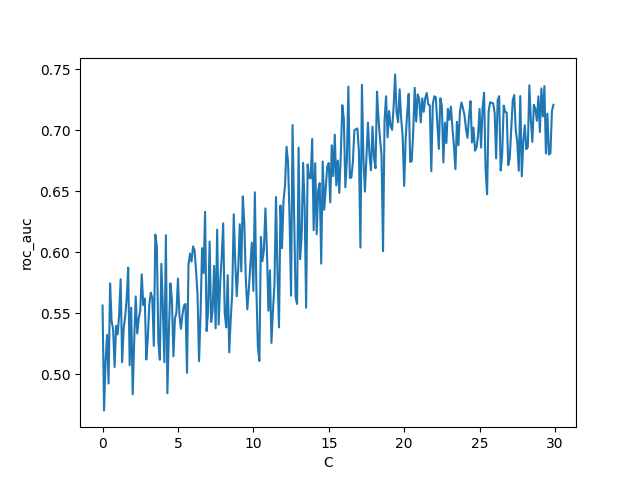
\includegraphics[width=0.8\textwidth]{svc}
\end{figure}
\begin{figure}[h!]
    \caption{MLPClassifier}
    \centering
    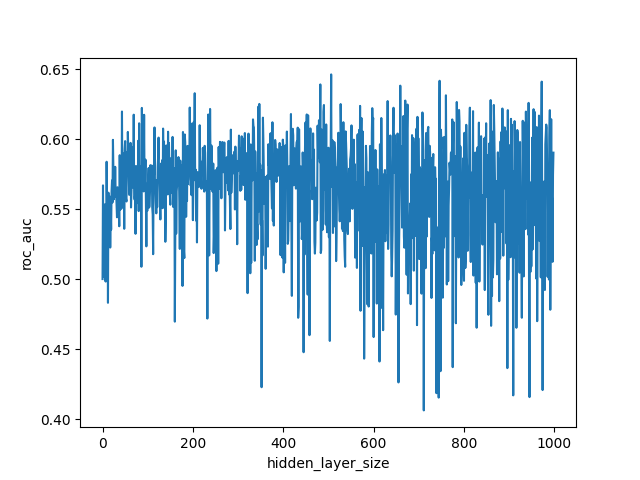
\includegraphics[width=0.8\textwidth]{mlp}
\end{figure}

Iz grafov vidimo, da je RFC daleč najboljši od izbranih algoritmov. Vidimo tudi, da je ročno nastavljena vrednost (80) in vrednost ugotovljena iz metaučenja (147) približno optimalna. Vidimo tudi, da je za SVC potrebno nastaviti $C>20$ in za kNN vsaj $k=80$. Obnašanje enoslojne nevronske mreže je preveč kaotično, da bi iz grafa kaj razbrali vendar vidimo, da se ne nauči dobro.

Na množici za treniranje dobita ročno nastavljanje in hyperopt dobre rezultate (93\% in 92\%). Na testni množici delata podobno dobro (93\% in 92\%), vendar opazimo, da je ročno nastavljanje bilo uspešnejše (izključimo naključnost tako, da povprečimo s 100 različnimi \verb|random_state|).
\begin{figure}[h]
    \caption{roc\_auc za ročno, hyperopt in openml z različnimi random stati}
    \centering
    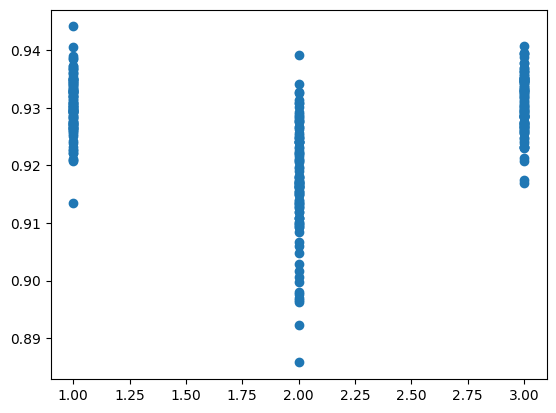
\includegraphics[width=0.8\textwidth]{scores}
\end{figure}
\end{document}